\section{Objectives of the analysis}
In this section, a presentation of the formal modeling activity has been created using the Alloy formal notation with the main goal of describing the domain and the properties of the system. 
The objective of this is to model and formally represent all the users (University, Student, Company, and regular User) and everything related to Internships and Internship Offers as well as the main constraints which regard all the entities mentioned.
\vspace{0.5cm}
\lstinputlisting[language=alloy]{Alloy/RASD_ALLOY.als}
\newpage
\section{Metamodels and Examples}
\subsection{General}
This model shows the entire system and all the complex relations among its parts. It can be quite useful to better understand how the single parts interact with each other.
\begin{figure}[H]
    \centering
    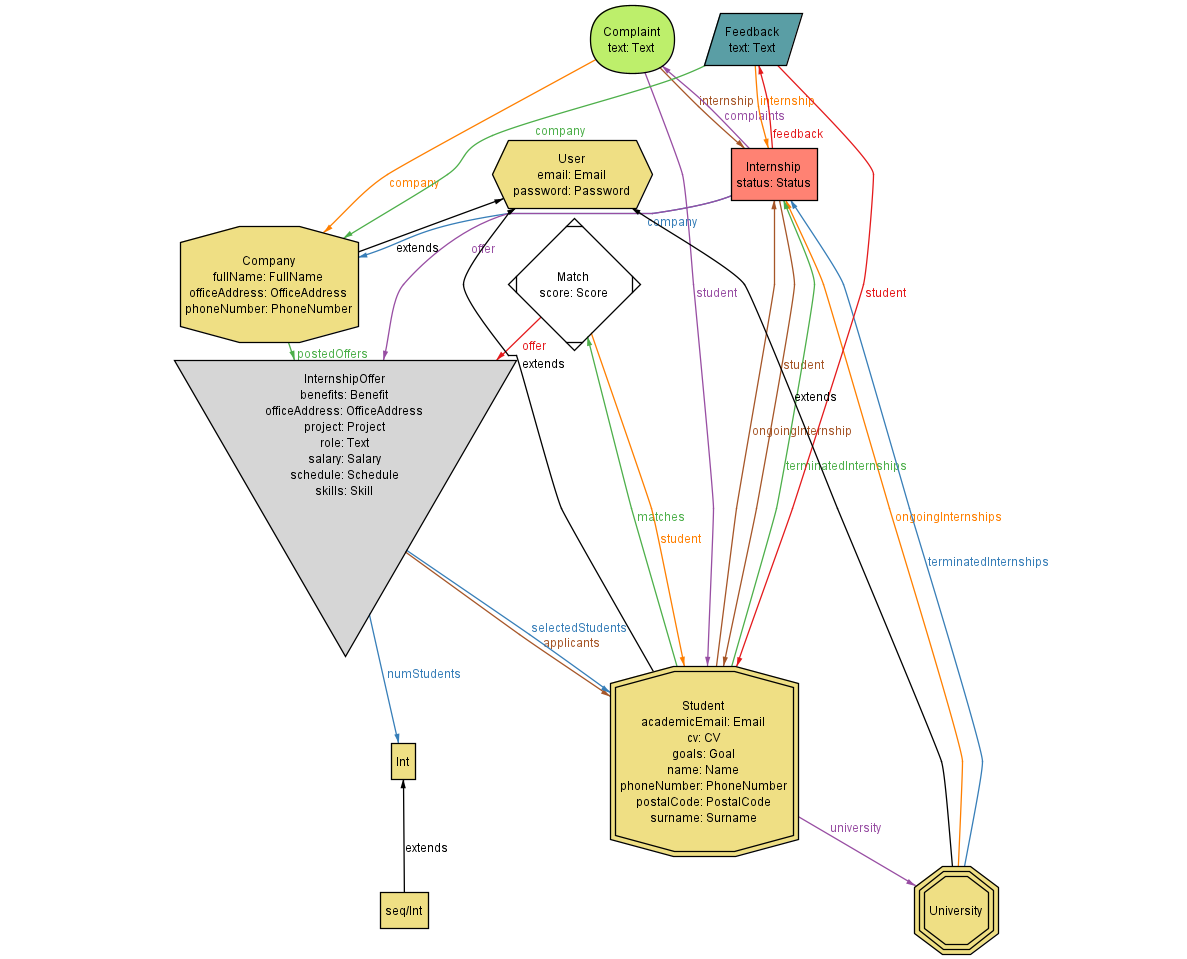
\includegraphics[width=0.75\linewidth]{Images/Alloy/metamodel.png}
    \caption{metamodel of the entire system }
    \label{fig:enter-label}
\end{figure}
\subsection{Users}
This model describes the basic properties of each user, independently from their type (University, Company, Student), without making any connection to other entities.
From this model the concept of the user who doesn't belong to one of the three groups that are able to interact with the platform is removed because it can not have relationships with any of the entities in the system.
\begin{figure}
    \centering
    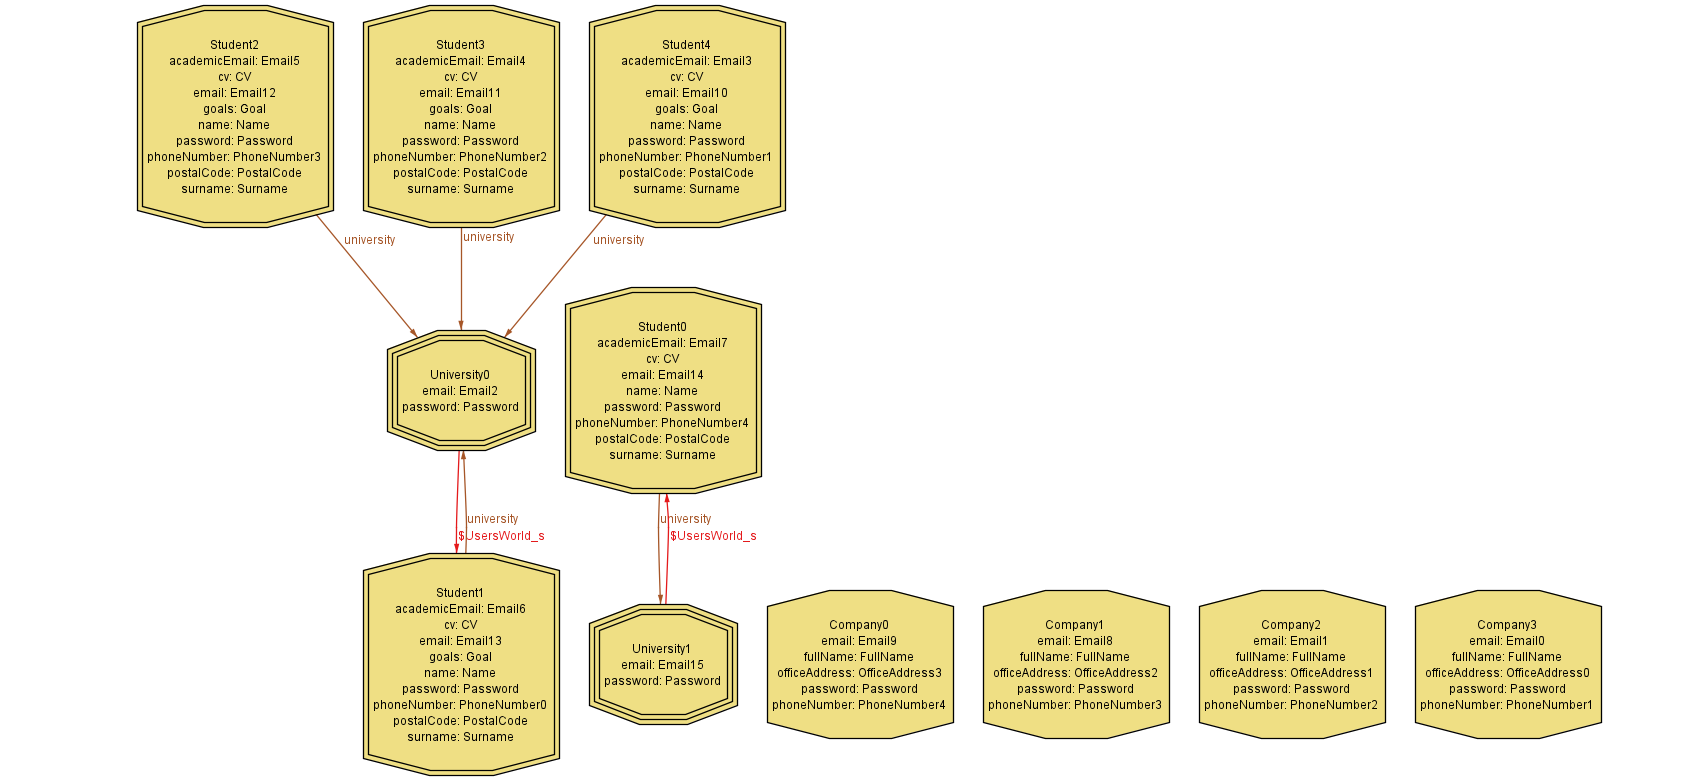
\includegraphics[width=0.5\linewidth]{Images/Alloy/Users.png}
    \caption{pred "UsersWorld" model}
    \label{fig:enter-label}
\end{figure}
\subsection{Internships and Internship offers}
This model describes the basic properties of the Internship and InternshipOffer entities.
\begin{figure}
    \centering
    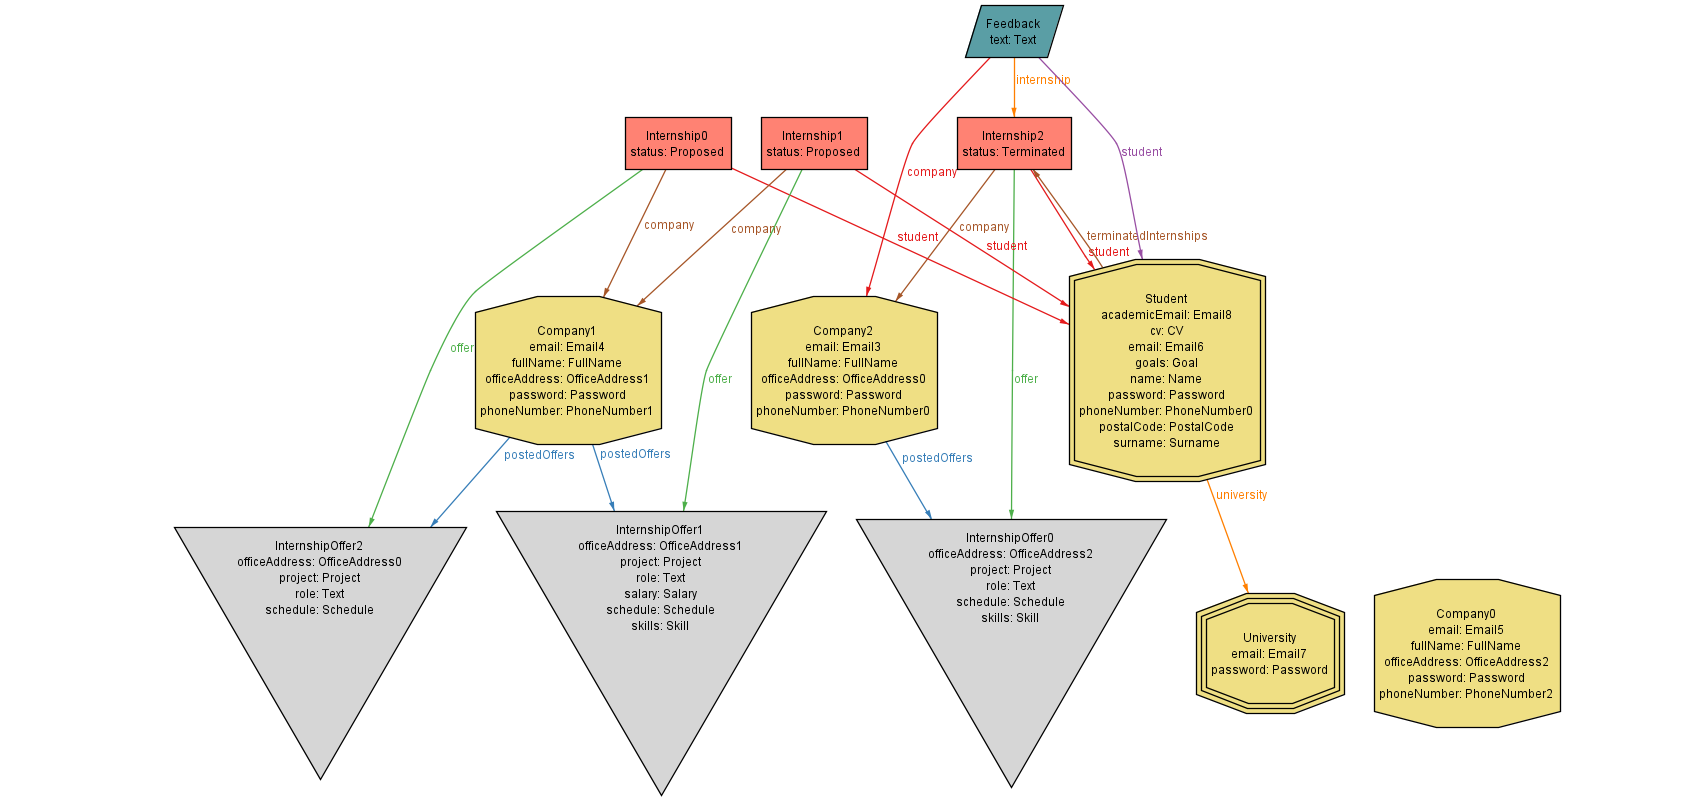
\includegraphics[width=0.5\linewidth]{Images/Alloy/Internship .png}
    \caption{pred "InternshipsWorld" model}
    \label{fig:enter-label}
\end{figure}
\subsection{Students applying to internships}
This model describes the interaction between Student, Internship and InternshipOffer when students start to apply to a specific offer. 
\begin{figure}
    \centering
    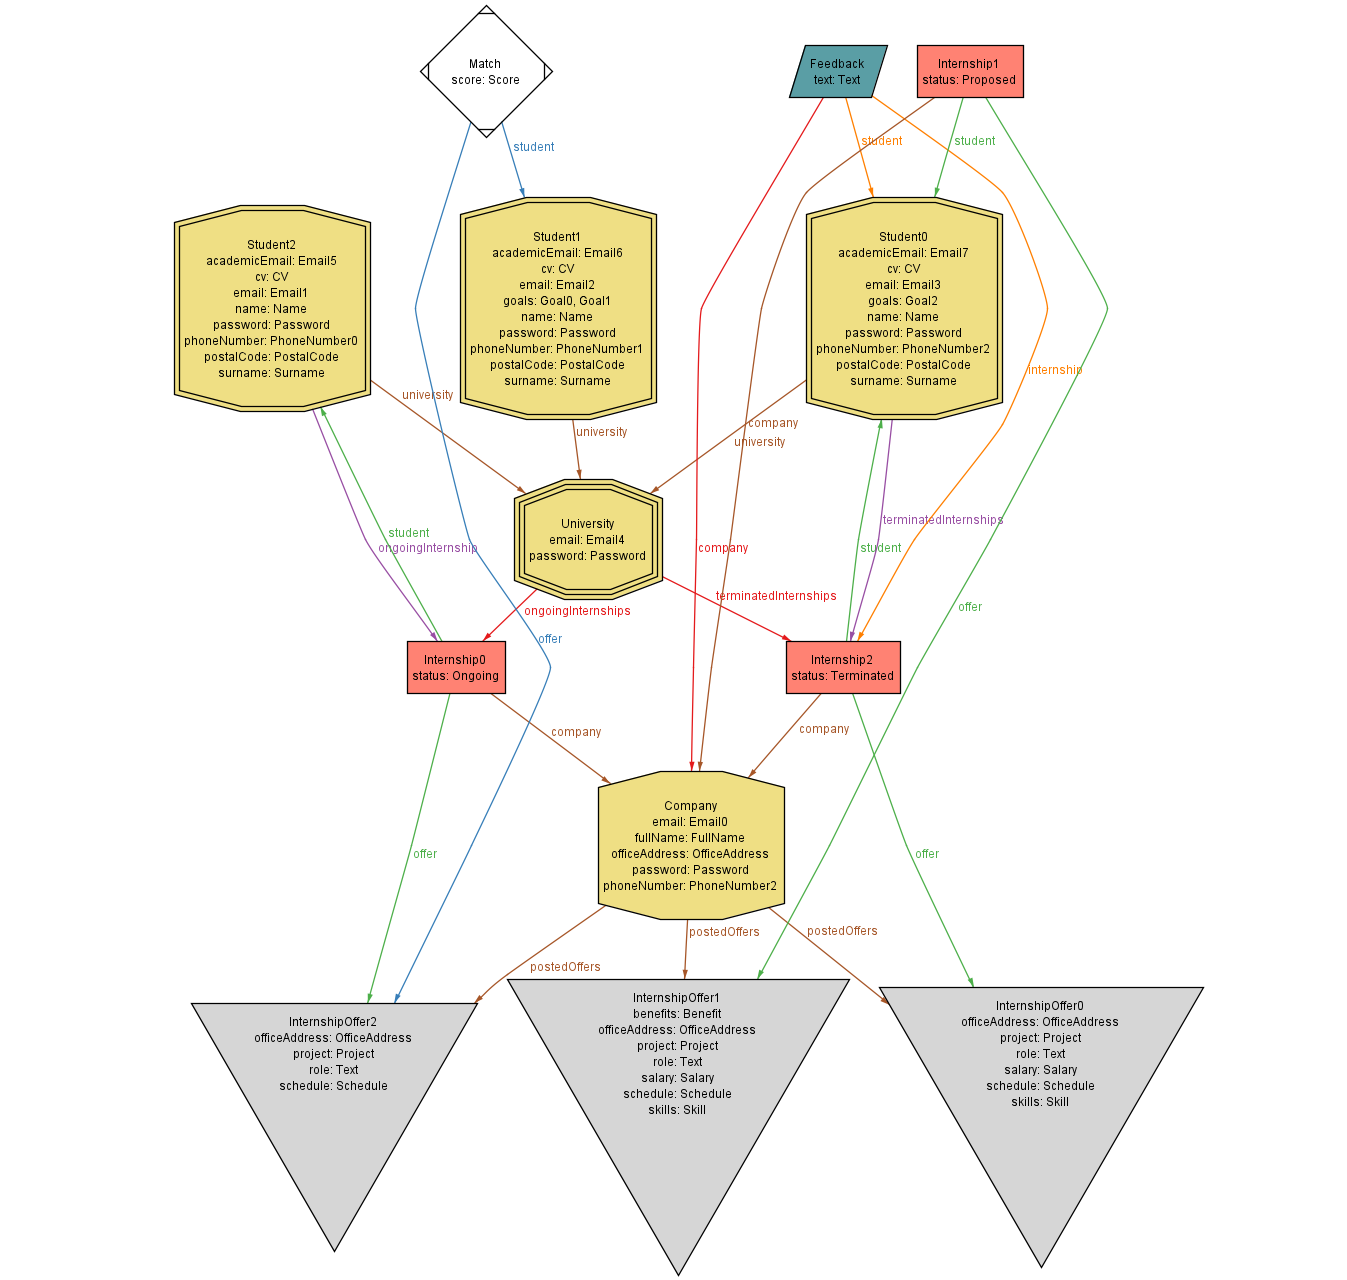
\includegraphics[width=0.5\linewidth]{Images/Alloy/Application.png}
    \caption{Pred "ApplicationWorld" model}
    \label{fig:enter-label}
\end{figure}
\subsection{Feedback and Complaint}
This model describes the relations between feedback and complaint entities and the other components of the system.
\begin{figure}
    \centering
    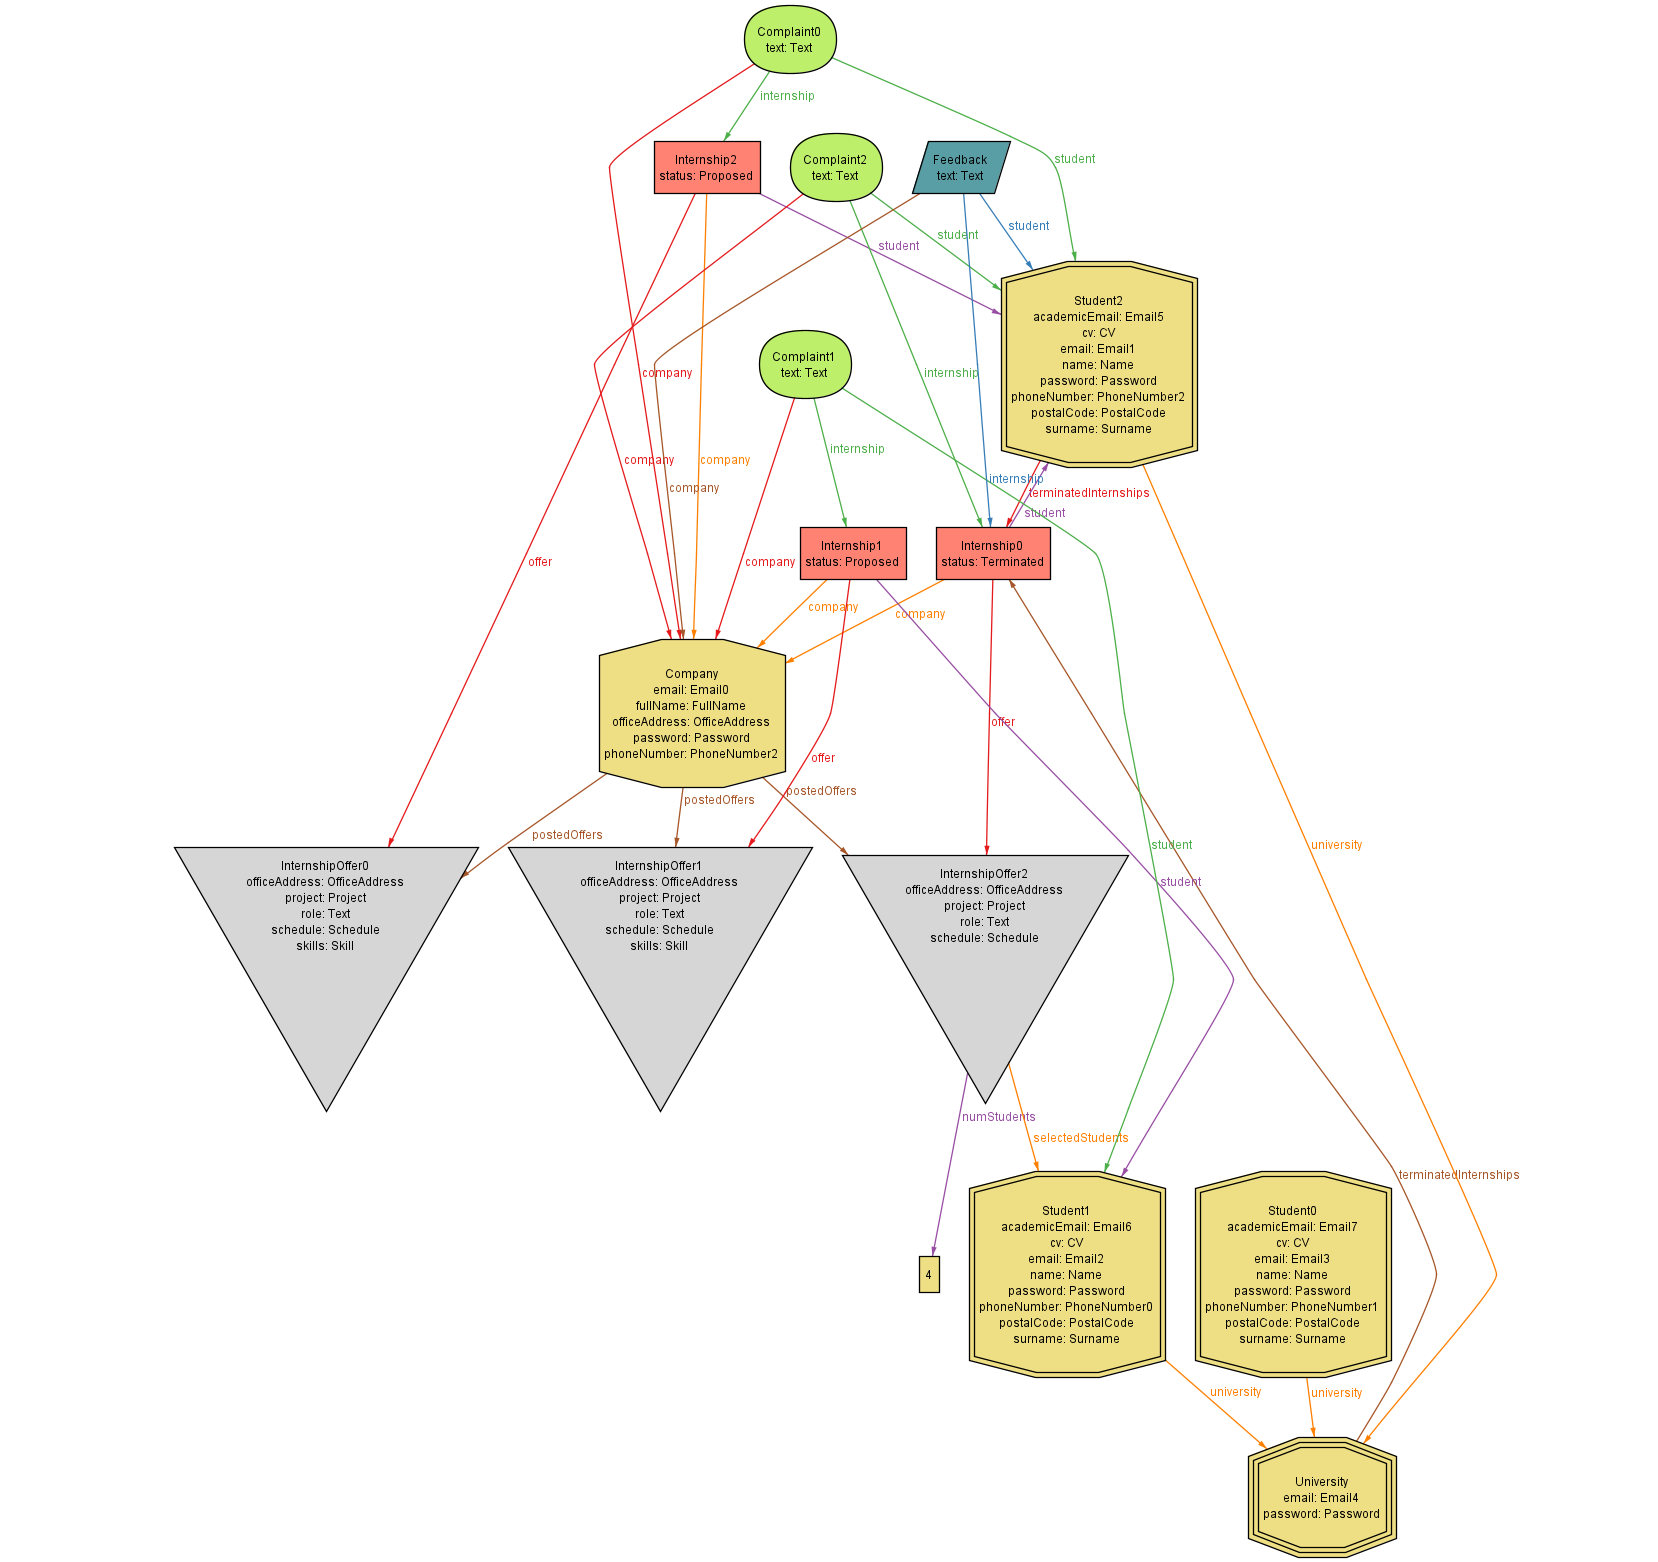
\includegraphics[width=0.5\linewidth]{Images/Alloy/ComplaintFeedback.png}
    \caption{Pred "FeedbackComplaintWorld" model}
    \label{fig:enter-label}
\end{figure}